We were primarily interested in two major results produced in \cite{Fiete}. First, we were interested the occurrence of long synfire chains with synchronous regular firing. We also investigated the paper's claim that STDP learning with \(w_{max} = W_{max}\) converged to scaled permutation matrices.

Though we tried to replicate the algorithm described in \cite{Fiete}, we were unable to produce a stable system with the provided inputs, so we had to tune the parameters a bit. We eventually found parameters at which burst rates were steady and believable. 

With the parameters we found, we were able to observe weaker versions of most of the observations in the paper. We found that weight matrices converged near scaled permutation matrices and we were able to observe some short sequences of firing chains, but we did not see the synchronous regular behavior exhibited in the paper.

Finally, we replaced STDP learning with Hebbian learning and demonstrated that the weights of a system undergoing Hebbian learning with soft and hard limits converged as closely or better to scaled permutation matrices than they did under STDP learning.

\subsection{Parameter Tuning}

Although our model was constructed to be identical to the model used in \cite{Fiete}, we were unable to use the same parameters as the paper. As an example, the paper claimed to set \(r_{in}\), external input, at 4 Hz. At 4 Hz, we were unable to get our system to fire at all! We assumed it was a typo (the rest of the parameters were given in terms of ms), and attempted running our simulation at 4000Hz. Even 4000Hz was not enough to get the system started, so we tried simulated annealing. The system began with 10000Hz of stimulation, which decreased steadily to 4000Hz. We did this again, but this time stopped at 6000Hz. The difference was striking (see figure \ref{burstSTDP}). 

\begin{figure}[H]
\centering
\begin{subfigure}[b]{0.49\textwidth}
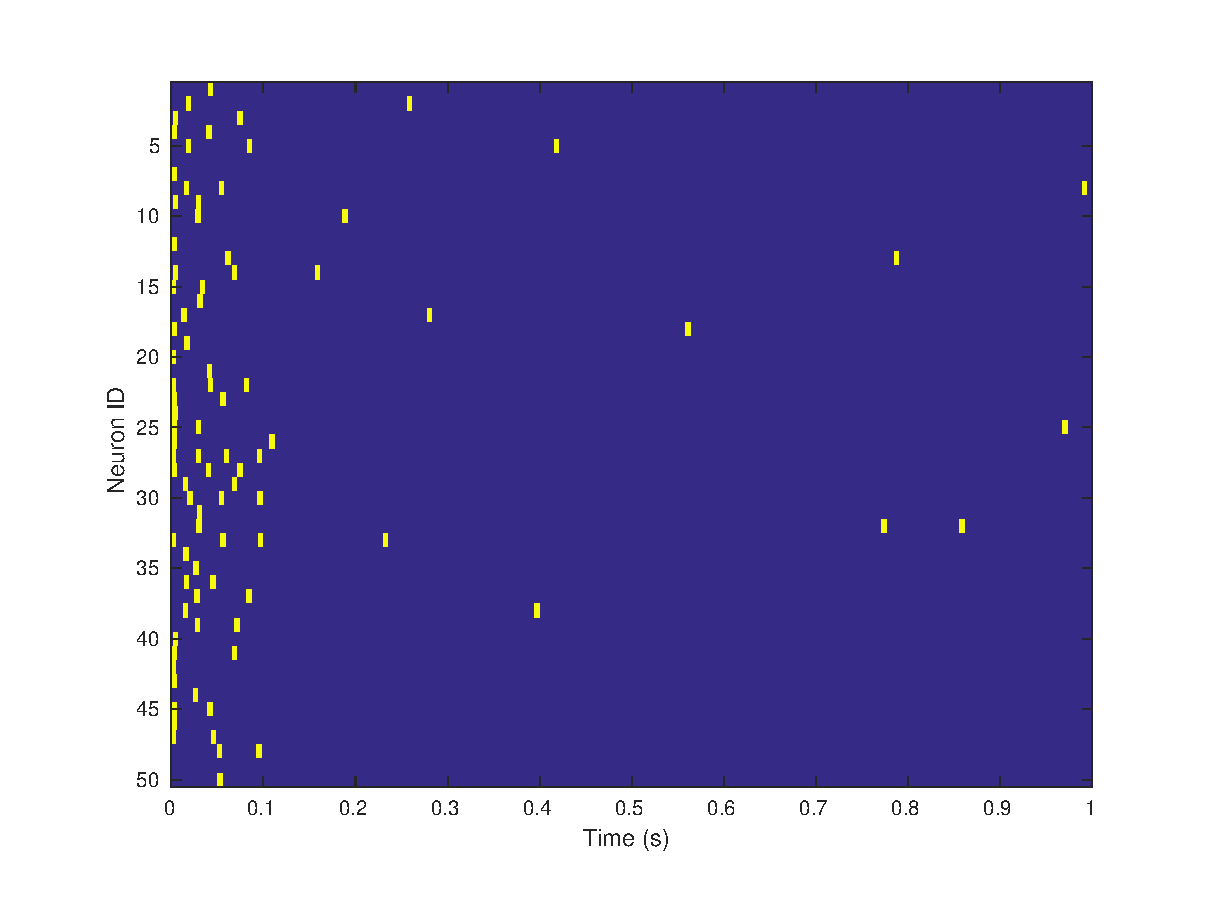
\includegraphics[width=\textwidth]{Burst_plot_4000Hz.eps}
\caption{4000 Hz}
\label{burstSTDP:4000}
\end{subfigure}
\,
\begin{subfigure}[b]{0.49\textwidth}
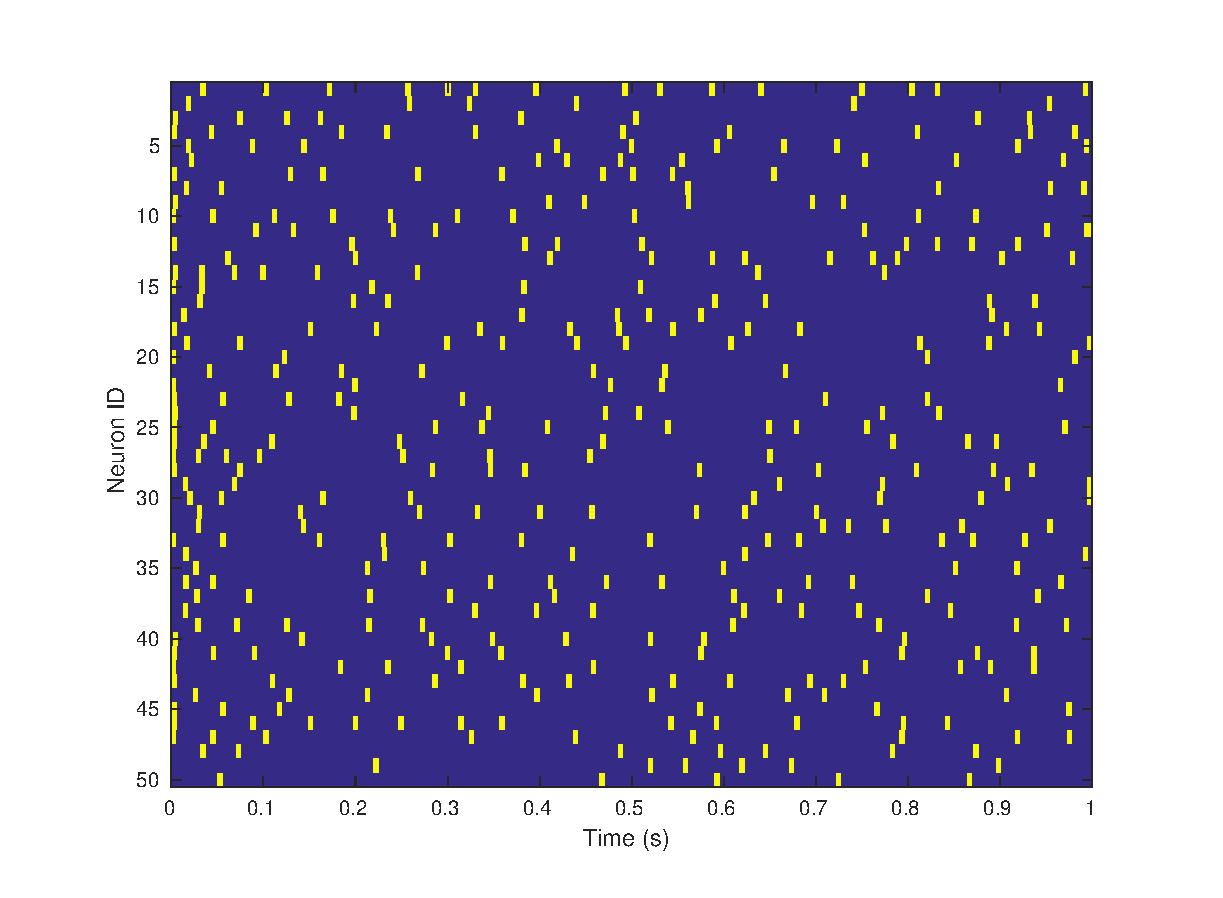
\includegraphics[width=\textwidth]{Burst_plot_6000Hz.eps}
\caption{6000 Hz}
\label{burstSTDP:6000}
\end{subfigure}
\caption{In figure 4 of \cite{Fiete}, the authors displayed a burst plot in which each neuron burst every 75 ms with high synchrony and regularity. We did not observe such synchrony in either plot, but the average frequency of firing in (b) was approximately 75 ms. Notice both systems exhibited exaggerated firing in the beginning. This was a consequence of simulated annealing.}
\label{burstSTDP}
\end{figure}

Beside \(r_{in}\), we spent a lot of time finding appropriate values for \(\eta\) and \(\epsilon\). 

\(\eta\) is the learning step-size. If \(\eta\) is too small, the weight matrix will not converge in a reasonable amount of time. If it is too large, whenever the weight matrix overshoots the soft limit, it will do so by a large margin, which will prompt large corrective measures, so convergence to a scaled permutation matrix (which is barely under the soft limit), will not be plausible.
 
\(\epsilon\) is the strength of the soft limit. If \(\epsilon\) is too small, then when the weight matrix passes the soft limit it will not experience very strong hLTD. This will have the effect of weakening heterosynaptic competition. If \(\epsilon\) is too large, then each time the weight matrix passes the soft limit, it will experience very strong hLTD. Because the scaled permutation matrix is on the border of the soft limit, having a large \(\epsilon\) will make any scaled permutation matrix an unstable critical point in our simulation.

To evaluate these, we ran the simulation on a large combination of parameter values for \(r_{in}, \eta\) and \(\epsilon\) (see figure \ref{Error_scatter: all}). For each of these, we tested convergence using an error function (see section 3.2). Then we isolated the product (\(\eta\epsilon\)) which seemed to yield the best results (see figure \ref{Error_scatter: constant product}).

\begin{figure}[H]
\centering
\begin{subfigure}[b]{0.49\textwidth}
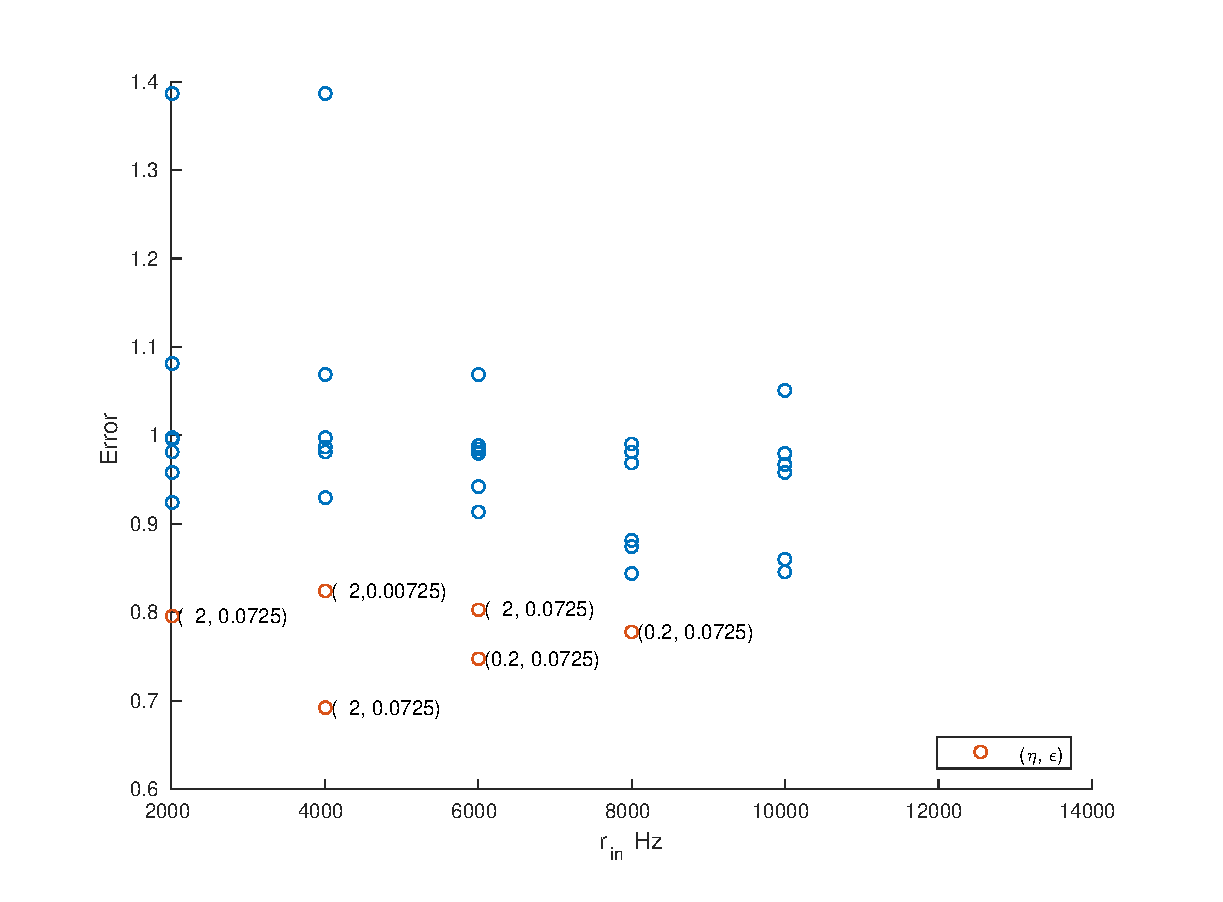
\includegraphics[width = \textwidth]{Error_Scatter_all.eps}
\caption{Errors of all simulations run}
\label{Error_scatter: all}
\end{subfigure}
\,
\begin{subfigure}[b]{0.49\textwidth}
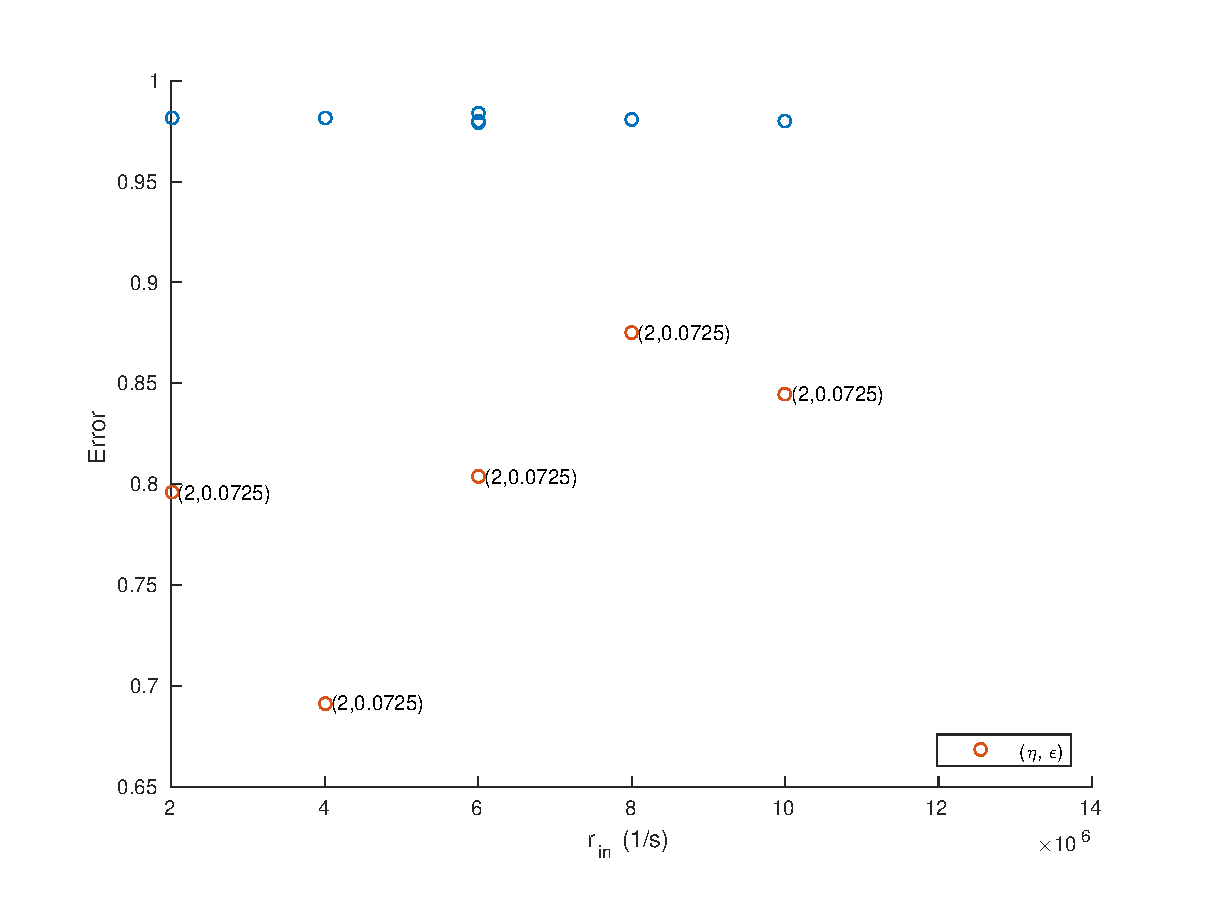
\includegraphics[width = \textwidth]{Error_Scatter_constantproduct.eps}
\caption{Errors of all simulations with \(\eta\epsilon = 0.145\)}
\label{Error_scatter: constant product}
\end{subfigure}
\label{Error_scatter}
\caption{Recall from \eqref{Learning-wrong} that in our implementation, \(\eta\) and \(\eta\epsilon\) are important tuning parameters for the rate of convergence. In all cases, we ran the algorithm for 50000 time steps with \(dt = 2\times 10^{-5}\)s. Notice that all error values are very high. (a) This is a plot of every simulation we ran. The best results are labeled. (b) This is a  plot of the subset of points from (a) where \(\eta\epsilon = 0.145\).}
\end{figure}

The best two combinations of parameters seemed to be \((r_{in},\eta,\epsilon) = \)(4000Hz, 2, 0.0725) and (6000Hz, 0.2, 0.0725). For the rest of the paper, we used these parameters unless otherwise noted.

Finally, we tried running a playback sequence with a fixed scaled permutation weight matrix. By symmetry, according to the model if one scaled permutation matrix is a stable point, then all of them must be. Therefore we fixed \(W\) to be a scaled permutation matrix. For convenience, we assumed this scaled permutation matrix was a large cycle. We ran it without modification to observe burst patterns for differing values of \(w_{max}\) (see figure \ref{Burst_no_learning}).

\begin{figure}[H]
\centering
\begin{subfigure}[b]{0.49\textwidth}
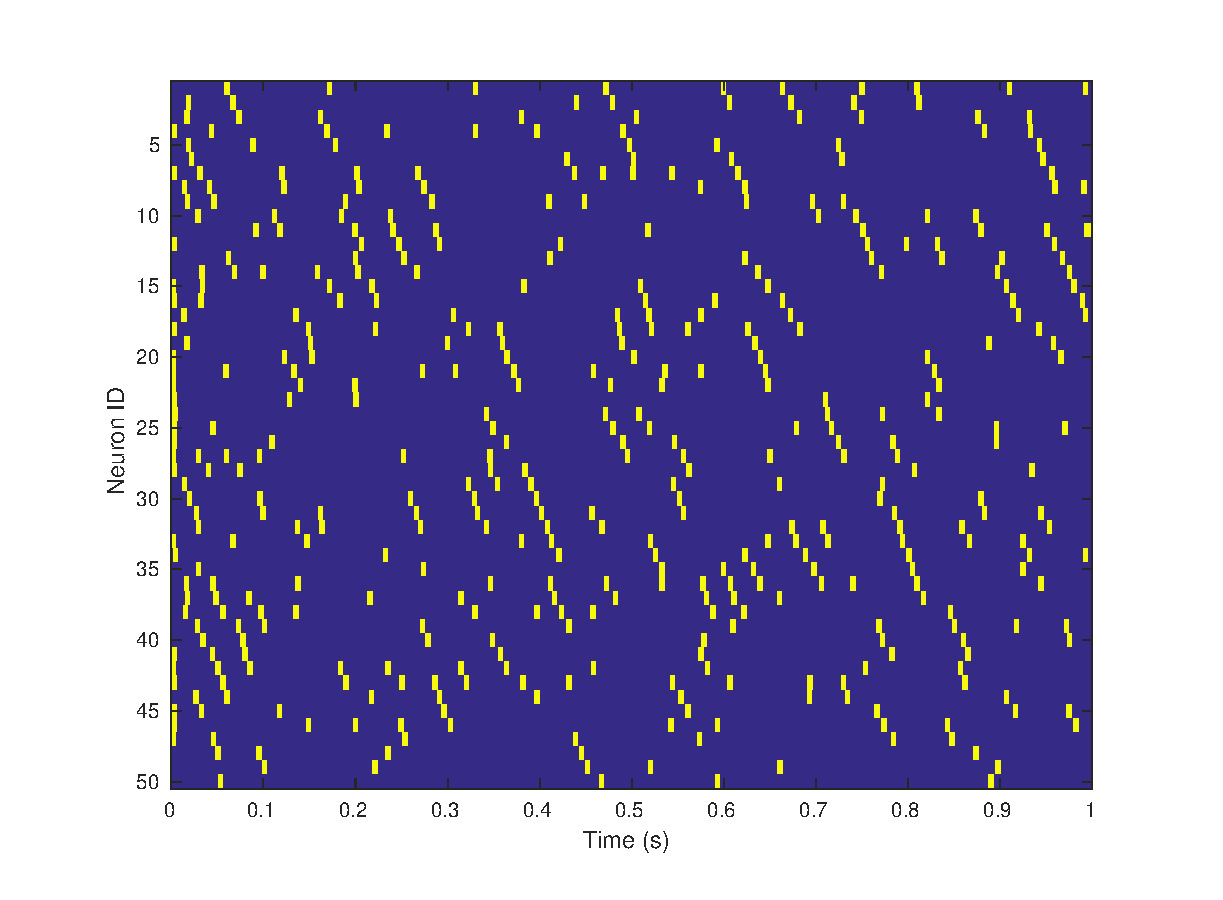
\includegraphics[width = \textwidth]{Burst_nolearning_perm_6000Hz_wmax0.14.eps}
\caption{Bursts without learning, \(w_{max} = 0.14\).}
\label{Burst_no_learning: 0.14}
\end{subfigure}
\,
\begin{subfigure}[b]{0.49\textwidth}
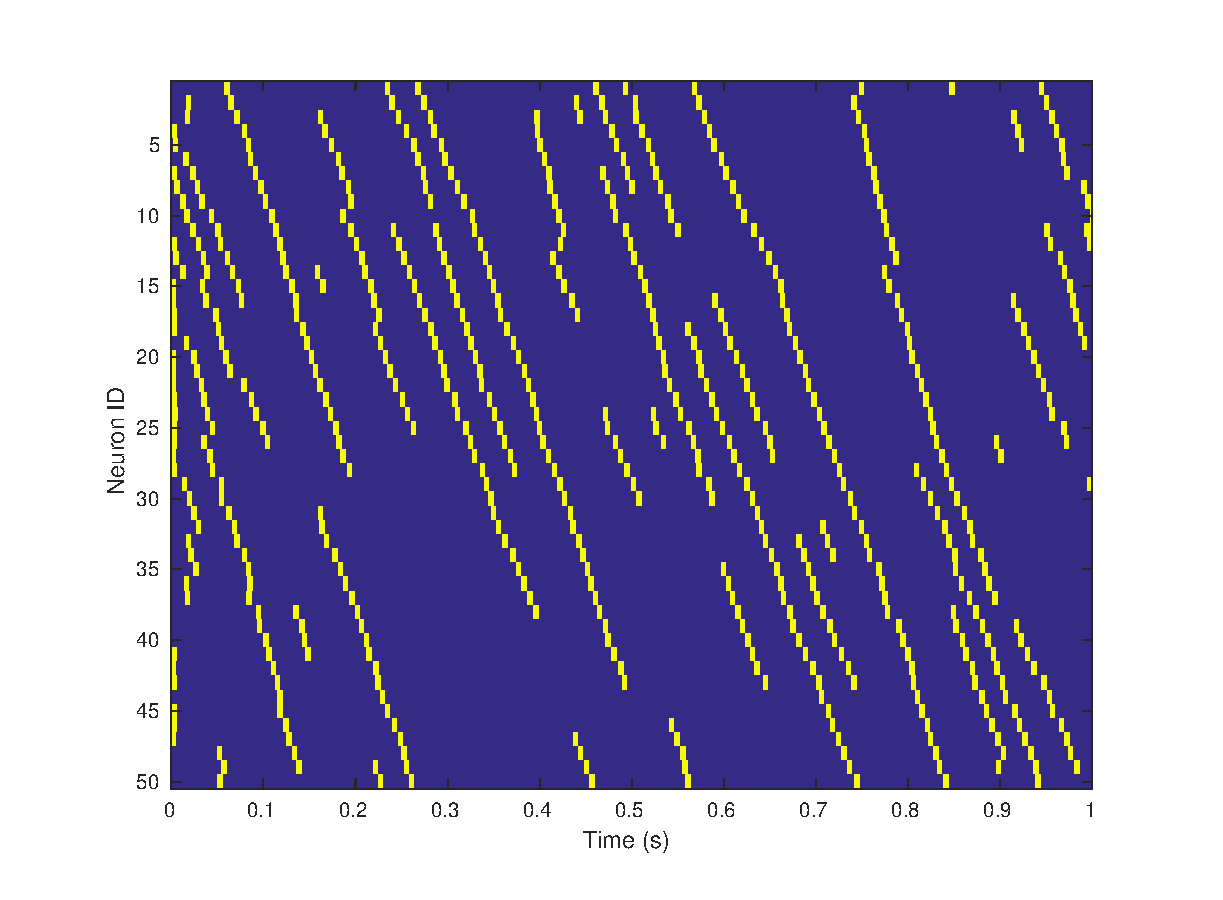
\includegraphics[width = \textwidth]{Burst_nolearning_perm_6000Hz_wmax0.3.eps}
\caption{Bursts without learning, \(w_{max} = 0.3\).}
\label{Burst_no_learning: 0.3}
\end{subfigure}
\\
\begin{subfigure}[b]{0.49\textwidth}
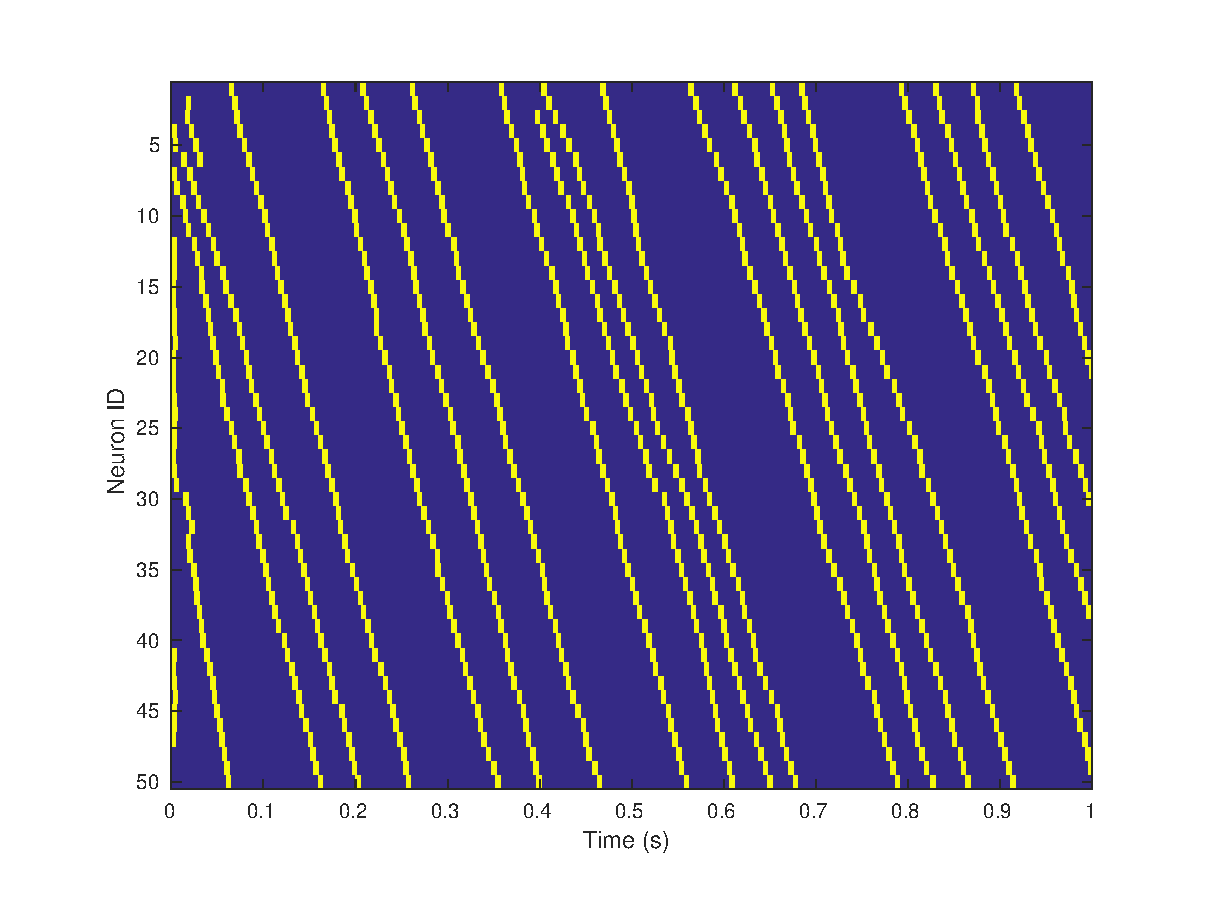
\includegraphics[width = \textwidth]{Burst_nolearning_perm_6000Hz_wmax0.5.eps}
\caption{Bursts without learning, \(w_{max} = 0.5\).}
\label{Burst_no_learning: 0.5}
\end{subfigure}
\,
\begin{subfigure}[b]{0.49\textwidth}
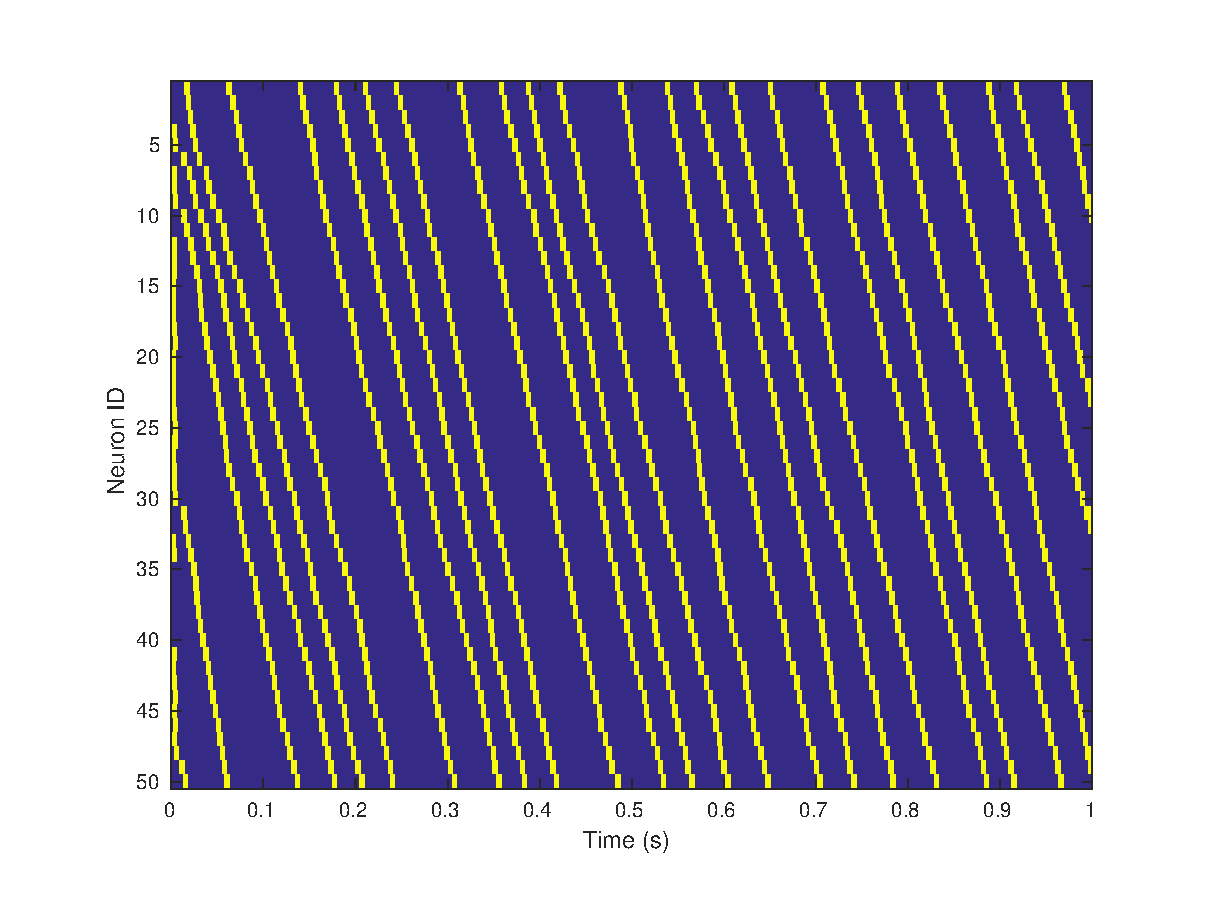
\includegraphics[width = \textwidth]{Burst_nolearning_perm_6000Hz_wmax0.7.eps}
\caption{Bursts without learning, \(w_{max} = 0.7\).}
\label{Burst_no_learning: 0.7}
\end{subfigure}
\caption{We ran the simulation for 50000 time steps at \(dt = 2\times 10^{-5}\)s with \(r_{in} = 6000\)Hz. As expected, for high values of \(w_{max}\), we witnessed high regularity, synchrony and long firing chains. At our default value of \(w_{max} = 0.14\) we witnessed a few small firing chains, but much more irregular firing.}
\label{Burst_no_learning}
\end{figure}

At our default \(w_{max}\) value, the IB model was unable to maintain the patterns of long sequential firing observed in \cite{Fiete}, however larger \(w_{max}\) values did display these patterns.

\subsection{Convergence and Stability}

Our IB model with STDP learning very quickly developed a stable bursting rate. Given up to about 4000Hz of external stimulation, this bursting rate was essentially 0, but for more stimulation the bursting rate was consistent. The neurons in the network constructed in figure 4 of \cite{Fiete}, on which our paper was based, bursted every 75 ms or so. From figure \ref{FR}, we can see that this corresponds to an external stimulation of slightly less than 8000Hz in our model.

\begin{figure}[H]
\centering
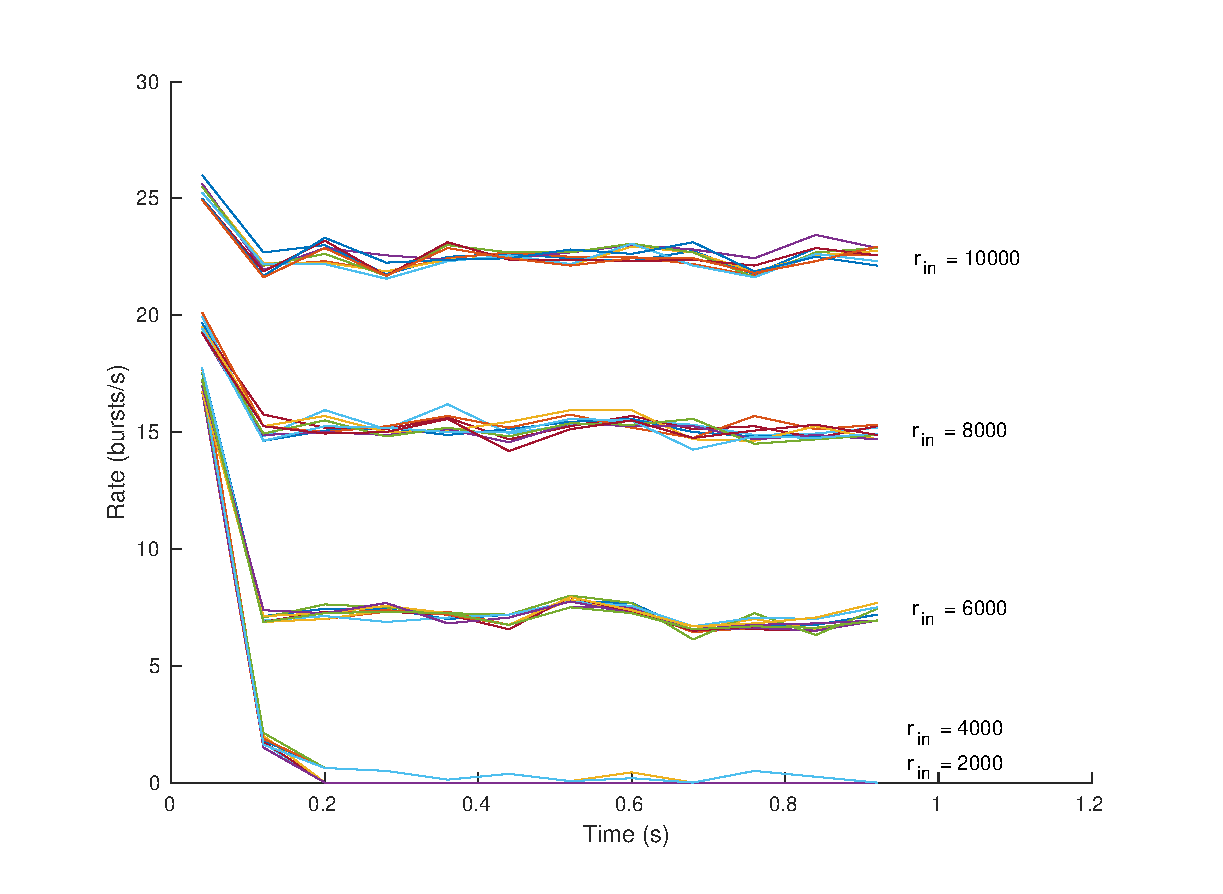
\includegraphics[scale = 0.7]{Firing_Rate_Binsize_80ms.eps}
\caption{The plot above measures the average firing rate of a neuron in the recurrent network over time over approximately 50 simulations. Notice that the average firing rate converges cleanly to different values dependent only on \(r_{in}\).}
\label{FR}
\end{figure}

From this we concluded that our base IB model was stable. The next thing we needed to test for was convergence of our weight matrix under STDP with soft and hard limits to a scaled permutation matrix. Recall that all permutation matrices \(P\) satisfy \(PP^T = I\). So, while we can visually inspect heat maps of \(W\) to see if it's close to a scaled permutation matrix, it is easier to look at how \(WW^T\) compares to \(w_{max}^2I\) (see figure \ref{Weights}).

\begin{figure}[H]
\centering
\begin{subfigure}[b]{0.49\textwidth}
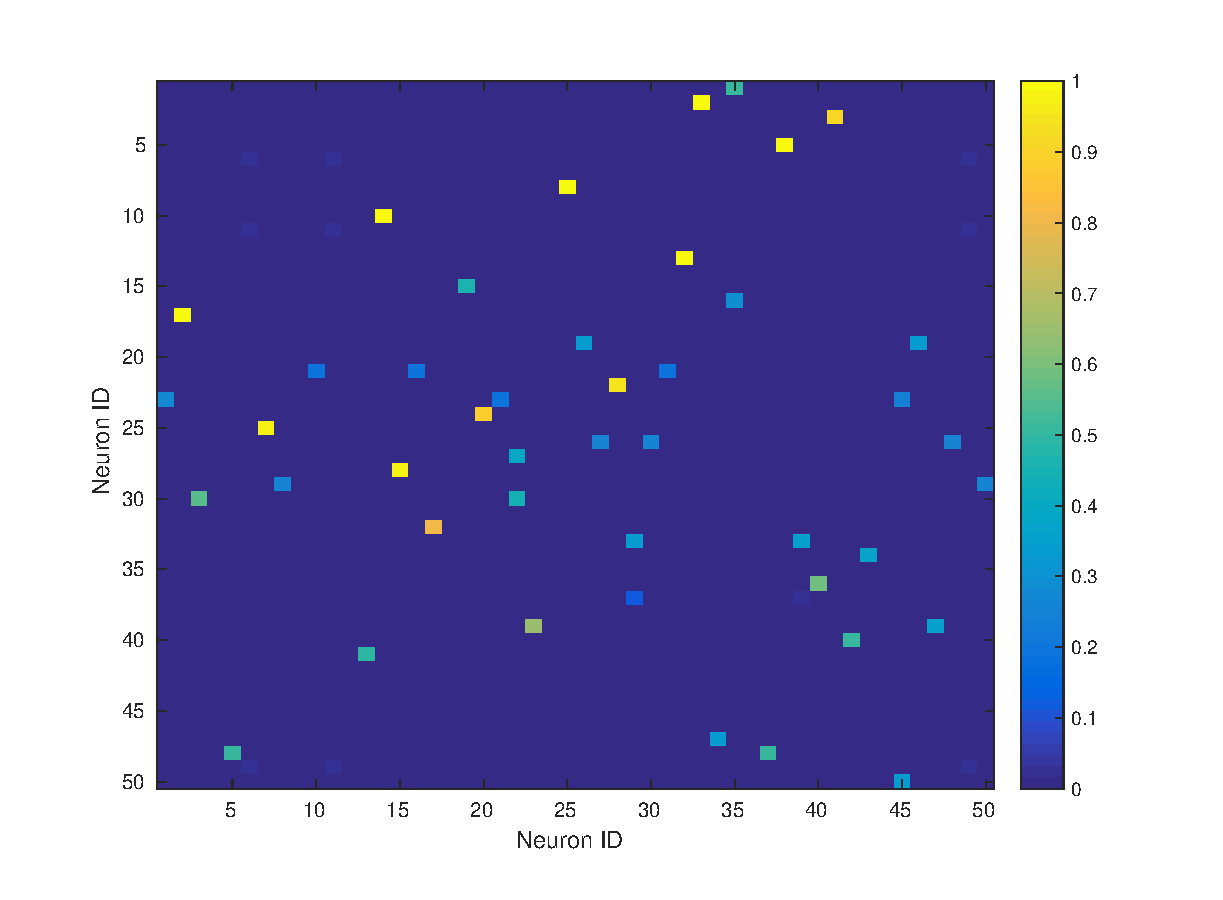
\includegraphics[width = \textwidth]{Weights_4000Hz.eps}
\caption{Weight matrix of 4000Hz external input with annealing}
\label{Weights: 4000Hz, basic}
\end{subfigure}
\,
\begin{subfigure}[b]{0.49\textwidth}
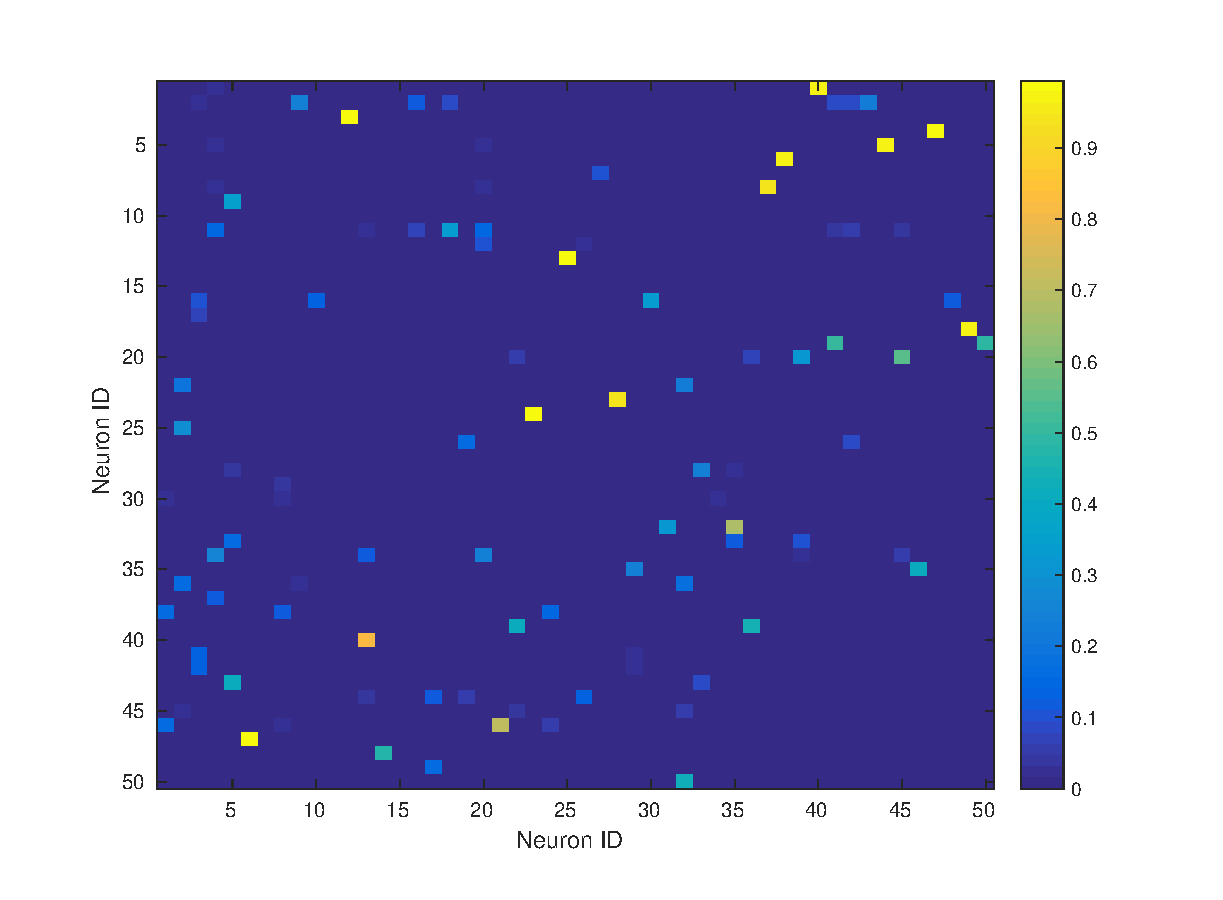
\includegraphics[width = \textwidth]{Weights_6000Hz.eps}
\caption{Weight matrix of 6000Hz external input with annealing}
\label{Weights: 6000Hz, basic}
\end{subfigure}
\\
\begin{subfigure}[b]{0.49\textwidth}
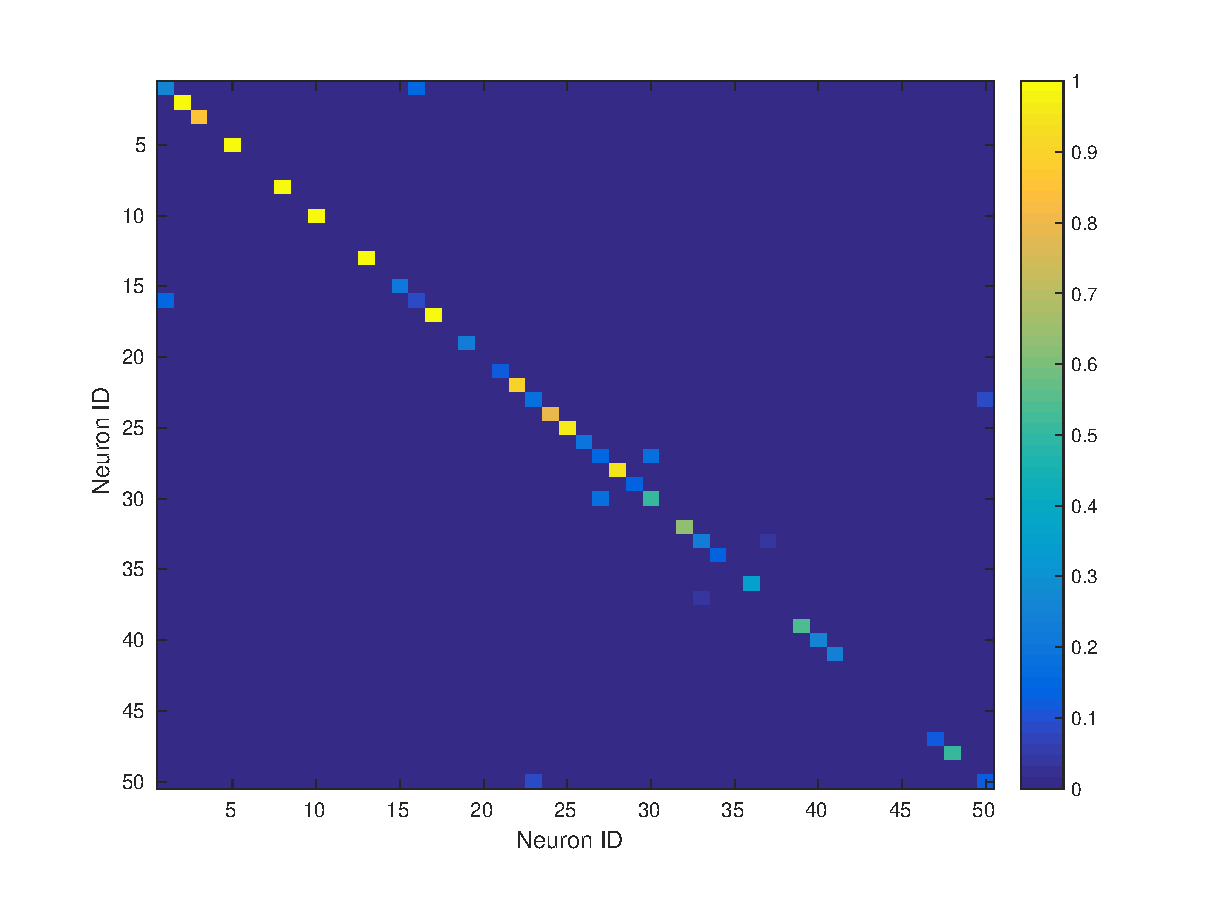
\includegraphics[width = \textwidth]{WW_4000Hz.eps}
\caption{\(WW^T\) of 4000Hz with annealing}
\label{Weights: 4000Hz, product}
\end{subfigure}
\,
\begin{subfigure}[b]{0.49\textwidth}
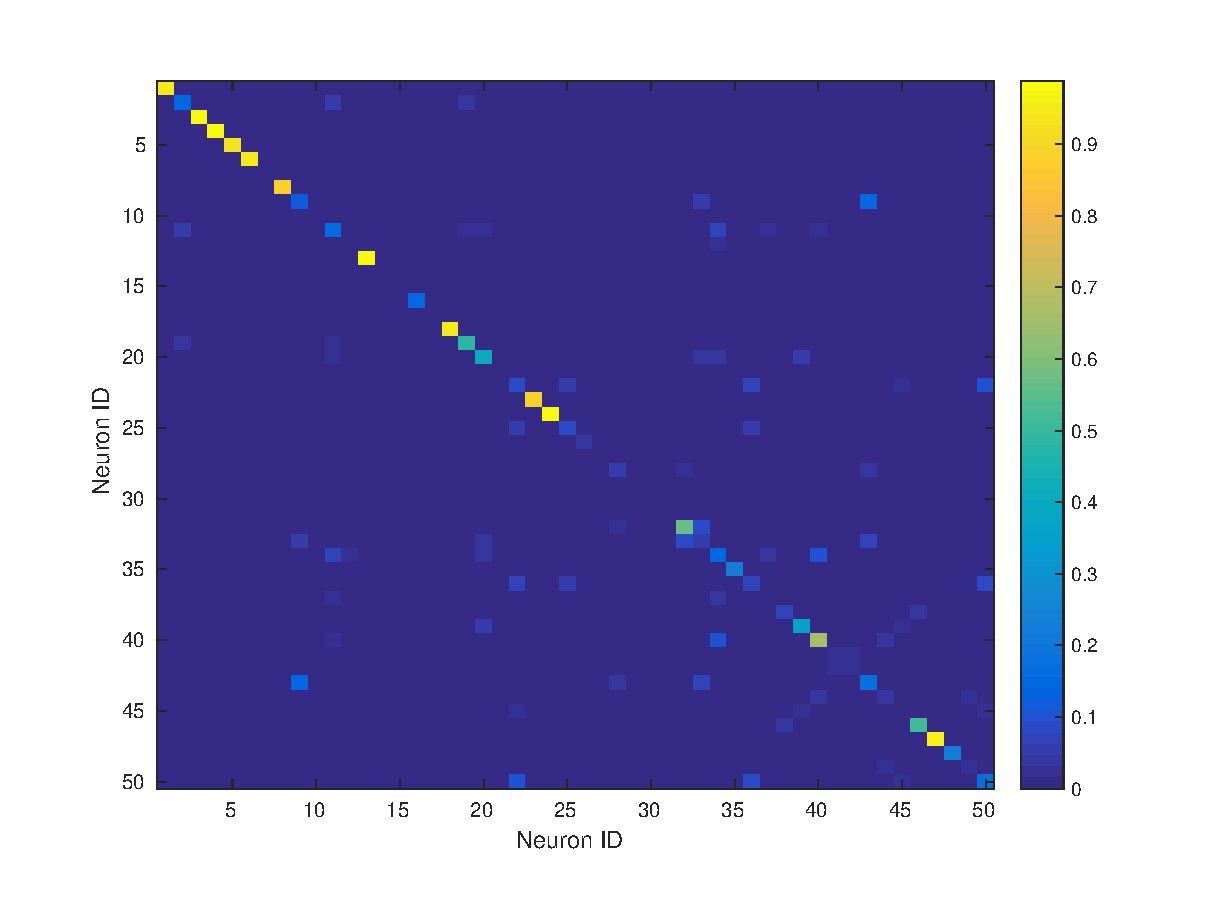
\includegraphics[width = \textwidth]{WW_6000Hz.eps}
\caption{\(WW^T\) of 6000Hz with annealing}
\label{Weights: 6000Hz, product}
\end{subfigure}
\caption{After running each simulation for 50000 time steps with \(dt = 2\times 10^{-5}\)s at 4000Hz and 6000Hz, we plotted the weight matrices, (a) and (b), and for each weight matrix \(W\) we plotted \(WW^T\), (c) and (d). While neither weight matrix converged perfectly to a scaled permutation matrix, each one looks like it is almost converged to a scaled permutation matrix.}
\label{Weights}
\end{figure}

While these figures seemed to confirm that the weight matrices were converging to scaled permutation matrices under STDP, it would be better to get some sense of convergence over time. To do this we introduce the following error function:

\[e(W) = \sum_{i,j=1}^N \left|WW^T - w_{max}^2I\right|_{ij}\]

This is the componentwise absolute difference between \(WW^T\) and \(PP^T\) for any permutation matrix scaled by \(w_{max}\). Notice that this measurement is actually a little generous, since permutation matrices are not the only square roots of the identity. However, it is simple to compute and if it is nonzero, then we are guaranteed that the weight matrix is not a scaled permutation matrix. See figure \ref{Error_over_time} for a plot of error over time. Notice that this error is unnormalized by \(w_{max}\), but that was not important here because we only used the error function with \(w_{max} = 0.14\).

\begin{figure}[H]
\centering
\begin{subfigure}[b]{0.49\textwidth}
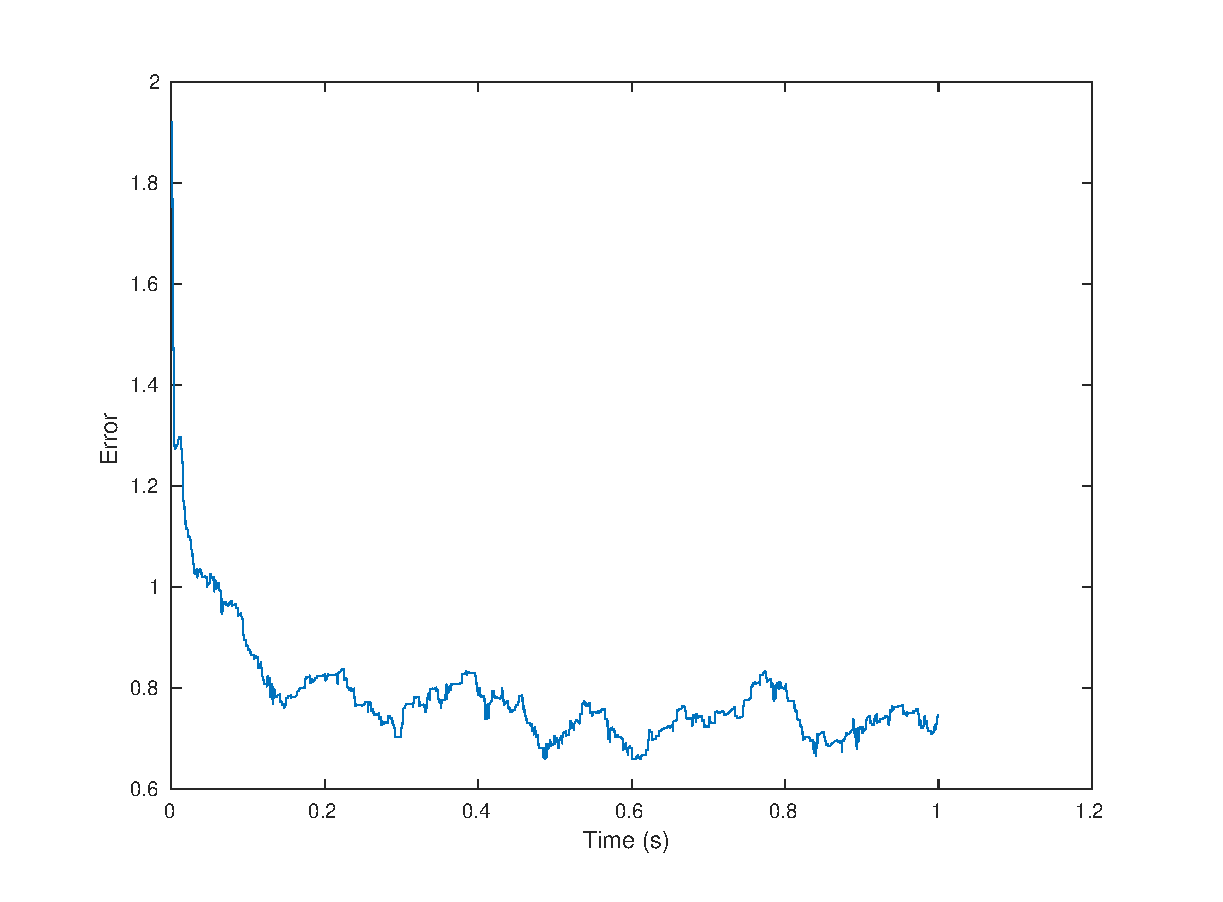
\includegraphics[width = \textwidth]{ErrorOverTime_6000Hz_normal.eps}
\caption{Plot of error in weights over time starting from a full connection weight matrix.}
\label{Error_over_time: normal}
\end{subfigure}
\,
\begin{subfigure}[b]{0.49\textwidth}
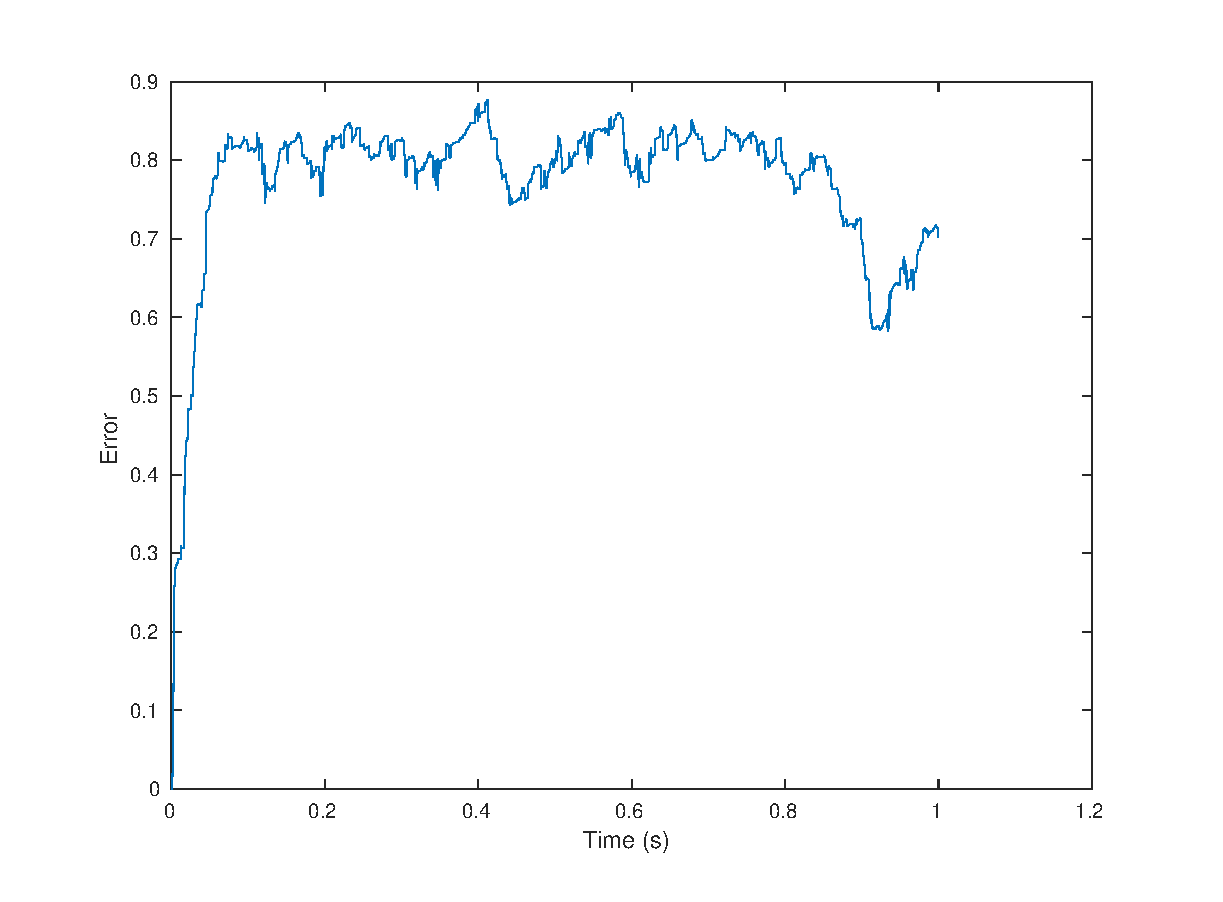
\includegraphics[width = \textwidth]{ErrorOverTime_6000Hz_Perm.eps}
\caption{Plot of error in weights over time starting from a scaled permutation weight matrix.}
\label{Error_over_time: permutation}
\end{subfigure}
\caption{(a) We ran a simulation where initial weights were all-to-all (minus diagonals) and uniform. (b) We ran a simulation where initial weights were already set to a scaled permutation matrix. In both cases the error roughly converged to about 0.7 with a fairly large variance.}
\label{Error_over_time}
\end{figure}

What's interesting is that after multiple runs with the same parameters we always converged to the same distance plus or minus some variance. There are a few explanations for this. As will be demonstrated in the next section, our implementation was flawed, and this caused most of the error. However, even with the proper implementation we observed a certain stable amount of error. See section 4 for more details.


\subsection{Hebbian Learning versus STDP}

Consider the following learning rule:

\[\od{W_{ij}}{t} = f(W_{ij},X) \text{ if } \sum_k W_{ik}, \sum_\ell W_{\ell j} \leq W_{max}\text{, otherwise }\]
\[\od{W_{ij}}{t} = f(W_{ij},X) - \delta\left(\left(\sum_k W_{ik} - W_{max}\right)^+ + \left(\sum_\ell W_{\ell j} - W_{max}\right)^+\right)\]
\[0\leq W_{ij} \leq w_{max} \quad W_{max} = w_{max}\]

Where \(X\) is a random variable and \(f(W,X) \geq 0\) and it is strictly increasing with respect to \(W\) with high probability.

Suppose \(W = w_{max}P\) where \(P\) is a permutation matrix. Consider \(W_Y = W + Y\), where \(Y\) is a random matrix such that for all \(i\) and \(j\), \(|Y_{ij}|< \epsilon\) for some small \(\epsilon \ll w_{max}\). Fix \(i,j\) so that \(W_{ij} = w_{max}\). Then there are three cases. First, both the rows and columns of \((W_Y)_{ij}\) satisfy the soft constraint. Then \((W_Y)_{ij}\) will increase until the soft limit is hit. If the soft limit is hit, assuming \(f\) increases strictly enough, \((W_Y)_{ij}\) should continue increasing until it hits the hard limit. At that point, all other elements in its rows and columns should tend to 0, or for sufficiently small \(\delta\), they may remain slightly positive.

While this treatment was far from rigorous, it does demonstrate that learning rules other than STDP may be combined with hLTD and hard limits to produce scaled permutation weight matrices. In particular, since higher synapse strength between neurons increases synchrony and firing rates, Hebbian plasticity may satisfy the conditions on \(f\) to produce scaled permutation weight matrices. To test this hypothesis, we ran a few simulations (see figure \ref{Compare}).

\begin{figure}[H]
\centering
\begin{subfigure}[b]{0.49\textwidth}
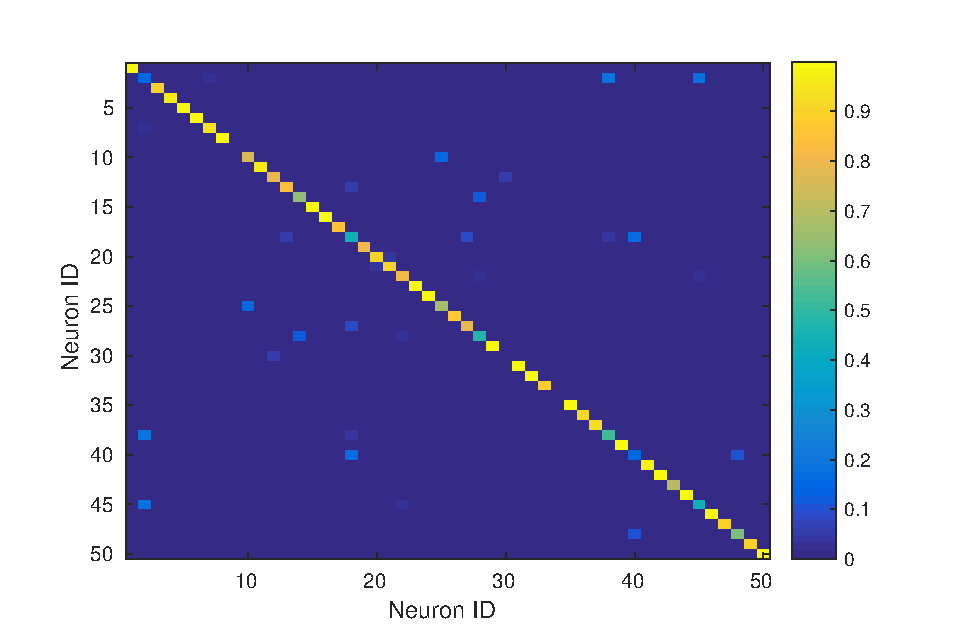
\includegraphics[width = \textwidth]{WW_6000Hz_Hebbian.eps}
\caption{\(WW^T\) matrix after Hebbian learning}
\label{Compare: WW_Hebbian}
\end{subfigure}
\,
\begin{subfigure}[b]{0.49\textwidth}
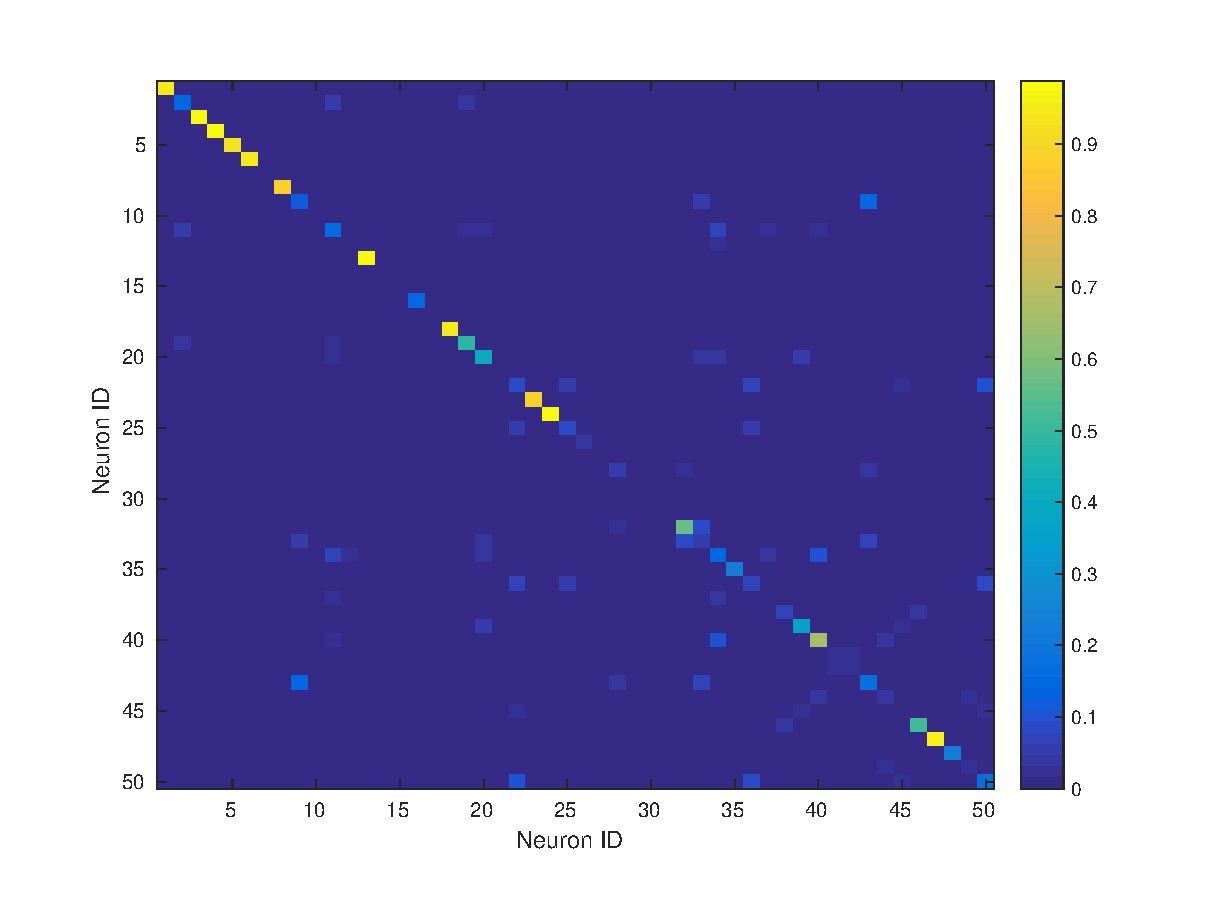
\includegraphics[width = \textwidth]{WW_6000Hz.eps}
\caption{\(WW^T\) matrix after STDP learning}
\label{Compare: WW_STDP}
\end{subfigure}
\\
\begin{subfigure}[b]{0.49\textwidth}
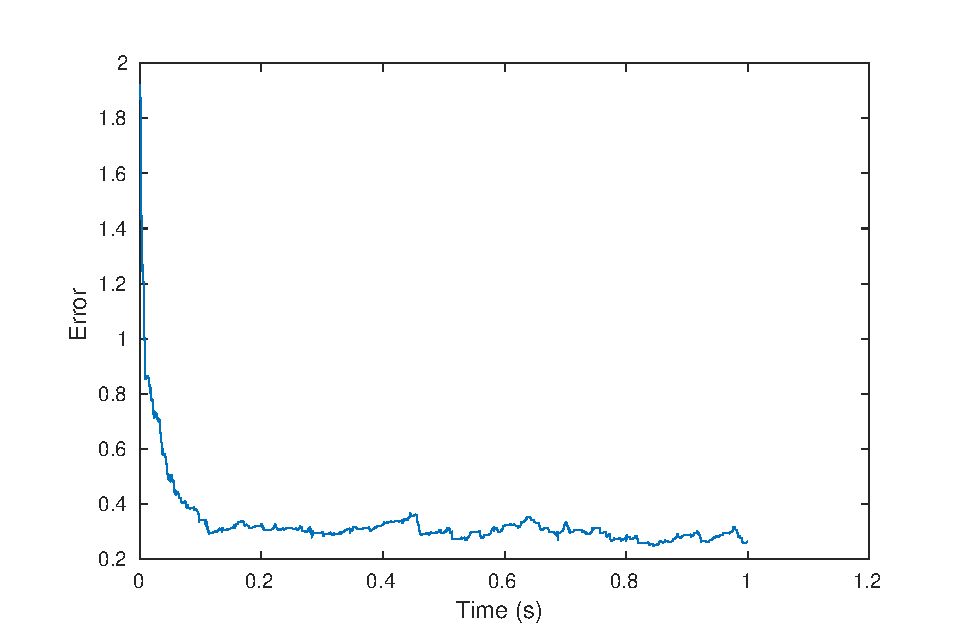
\includegraphics[width = \textwidth]{ErrorOverTime_6000Hz_Hebbian.eps}
\caption{Error over time of Hebbian Learning}
\label{Compare: EoT_Hebbian}
\end{subfigure}
\,
\begin{subfigure}[b]{0.49\textwidth}
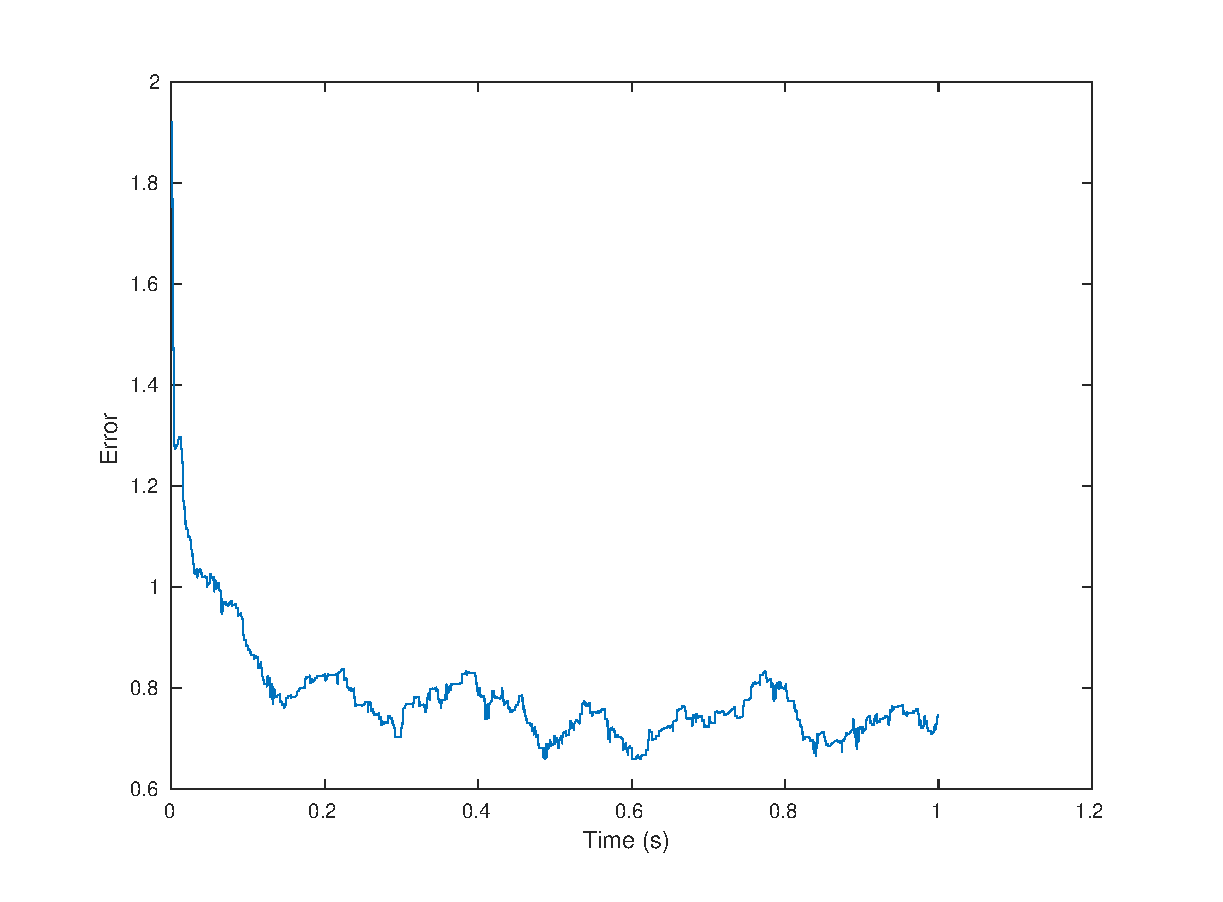
\includegraphics[width = \textwidth]{ErrorOverTime_6000Hz_normal.eps}
\caption{Error over time of STDP Learning}
\label{Compare: EoT_STDP}
\end{subfigure}
\\
\begin{subfigure}[b]{0.49\textwidth}
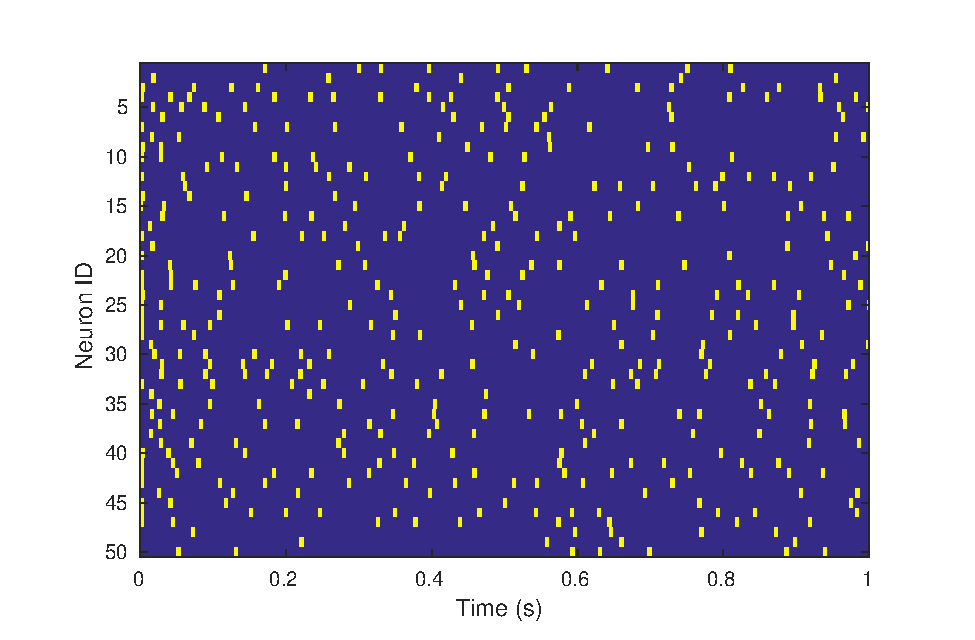
\includegraphics[width = \textwidth]{Burst_plot_6000Hz_Hebbian.eps}
\caption{Burst history of Hebbian plot}
\label{Compare: BH_Hebbian}
\end{subfigure}
\,
\begin{subfigure}[b]{0.49\textwidth}
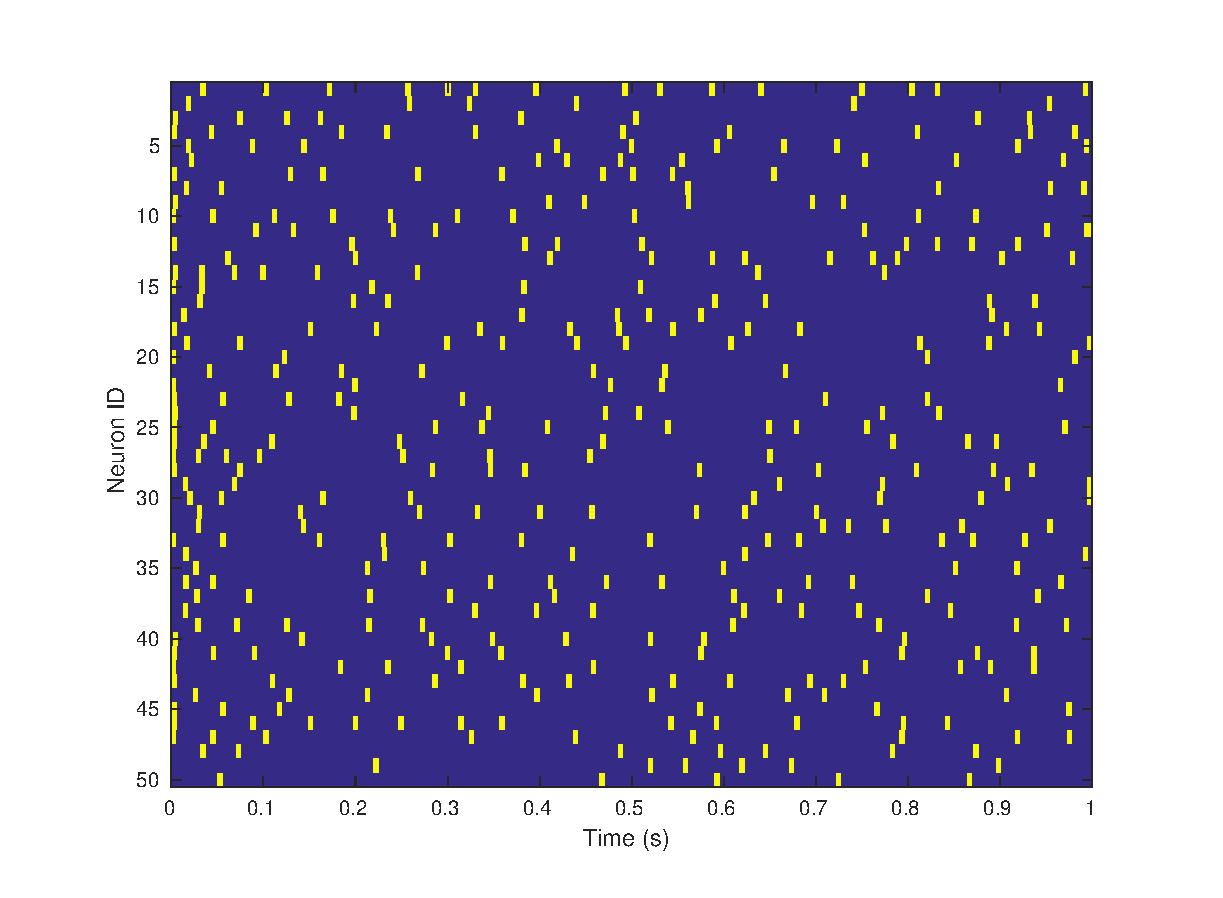
\includegraphics[width = \textwidth]{Burst_plot_6000Hz.eps}
\caption{Burst history of STDP plot}
\label{Compare: BH_STDP}
\end{subfigure}
\caption{Comparison of STDP and Hebbian learning simulations at 6000Hz of input}
\label{Compare}
\end{figure}

From figure \ref{Compare}, it's clear that the weight matrix of the network with Hebbian learning converged more closely to a scaled permutation matrix than the STDP equivalent and with less variability. However, both simulations demonstrated similar levels of synchronized regular burst output and similar occurrence of synfire chains. This provides strong evidence that Hebbian learning with hLTD is sufficient to reproduce the results of \cite{Fiete}.